\chapter{Mindmap}
\authortoc{\bastian}{\chapterident}
\begin{figure}[!ht]
  \centering
  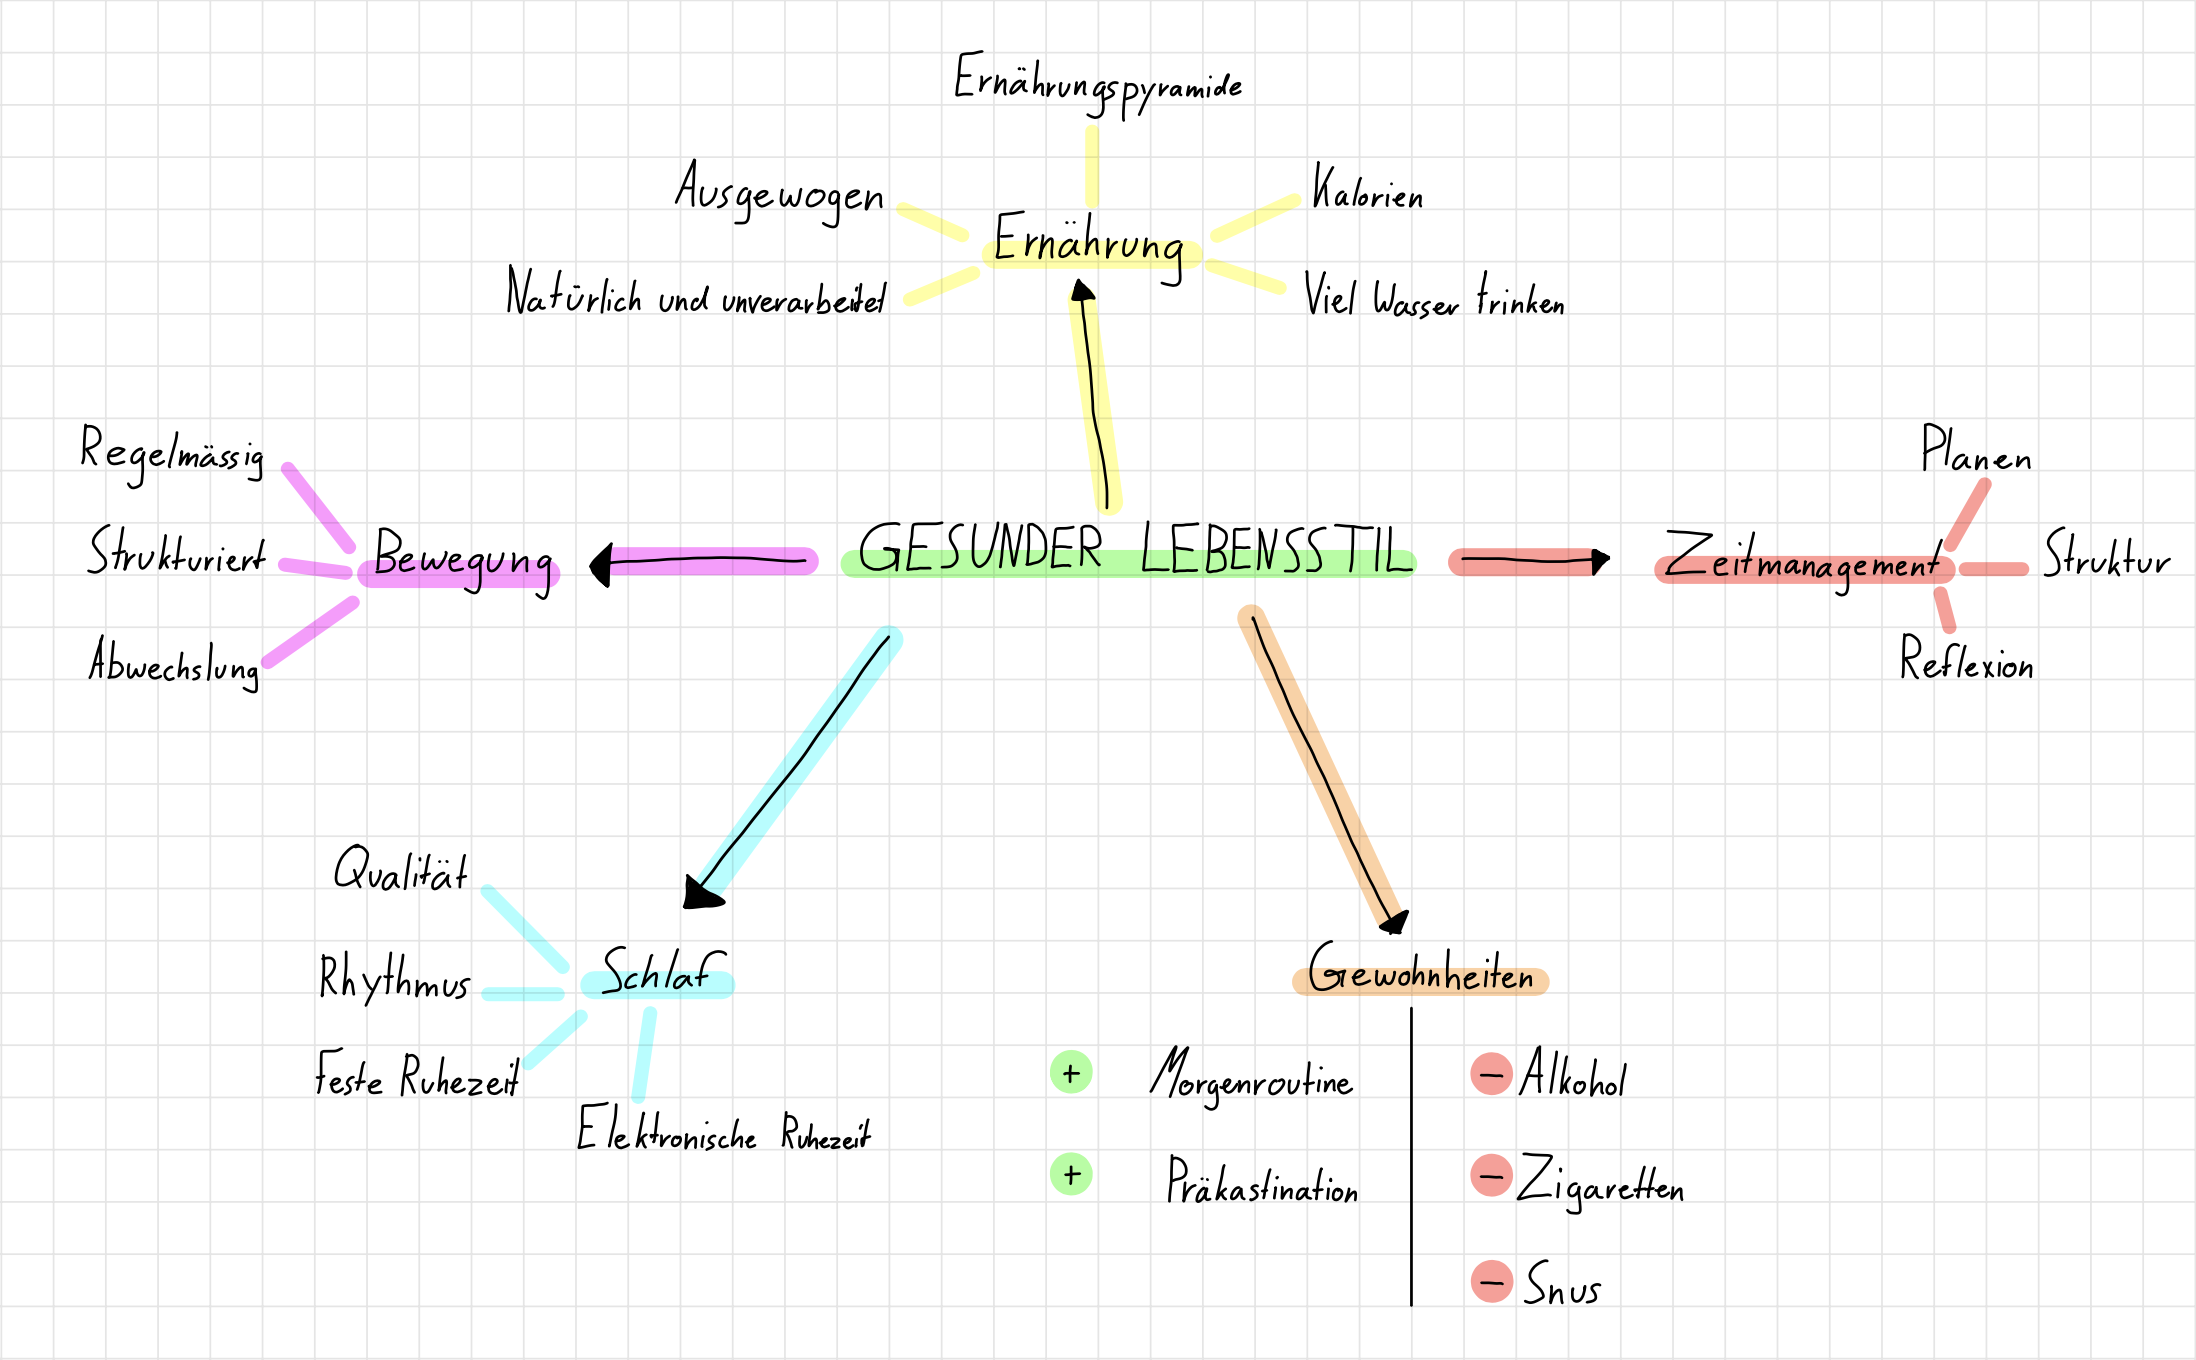
\includegraphics[width=.9\linewidth]{./images/mindmap.png}
  \caption[Ein von uns digital erstelltes Mindmap]{Mindmap gesunder Lebensstil}
  \label{fig:mindmap}
\end{figure}
Wir haben uns zusammengesetzt und überlegt, was alles zu einem gesunden Lebensstil gehört. Dafür haben wir ein Mindmap erstellt, welches unsere Überlegungen widerspiegelt. Dabei haben wir fünf Themen gewählt, welche unserer Meinung nach die wichtigsten für einen gesunden Lebensstil sind. Diese Themen sind zum einen die Bewegung, zum anderen die Ernährung, das Zeitmanagement, die Gewohnheiten und ebenfalls der Schlaf. Zu diesen Punkten haben wir schliesslich einige Ideen gesammelt, welche unserer Meinung nach wichtig waren.
\begin{enumerate}
  \item Bei der Bewegung haben wir als wichtige Unterpunkte die Regelmässigkeit, die Strukturierung und die Abwechslung gewählt. Unsere Überlegung war dabei, dass wir eine Routine hereinbringen, uns dabei mehrmals wöchentlich auf eine sportliche Art bewegen und dies auch abwechslungsreich gestalten. Damit meinen wir, dass man nicht immer das Gleiche machen muss, wie z. B. Krafttraining, sondern auch Ausdauertraining oder je nachdem auch andere Arten von Training oder Bewegung zur Förderung unserer Gesundheit. Zudem setzt man mehr Muskelreize, wenn das Training auf verschiedene Art die Muskulatur beansprucht. Das sorgt für eine gute und qualitativ hochwertige Muskulatur.
  \item Bei der Ernährung haben wir fünf wichtige Unterthemen gewählt: Natürlich und unverarbeitet, ausgewogen, Ernährungspyramide, Kalorien und viel Wasser trinken. Dabei haben wir uns gedacht, dass man möglichst wenig verarbeitete Produkte essen sollte und stattdessen lieber auf unverarbeitete Produkte setzt. Ein Beispiel dafür wäre eine Wurst und eine Pouletbrust. Beides ist Fleisch, jedoch ist das eine verarbeitetes Fleisch und das andere unverarbeitet. Mit der Verarbeitung wird das Produkt ungesünder. Es ist auch sehr wichtig, dass die Ernährung ausgewogen ist, was heisst, dass sie vielseitig und von allem etwas enthalten sollte. Ebenfalls kann man sich auch nach der Ernährungspyramide richten, welche vorgibt, wie viel Lebensmittel man konsumieren sollte, um sich ausgeglichen und gesund zu ernähren. Auch die Kalorienanzahl ist wichtig, denn gesund ist nicht gleich kalorienarm. Es gibt viele gesunde Lebensmittel, welche aber sehr viele Kalorien haben. Trotzdem sollte man schauen, dass man seine Tagesration an Kalorien einteilt und nicht zu viel einnimmt. Zum Schluss haben wir die simpelste Sache und das wäre viel Wasser trinken. Dafür sollten auf andere Getränke wie zum Beispiel Süssgetränke verzichtet werden.
  \item Als nächsten Punkt haben wir das Zeitmanagement mit den Unterthemen Planung, Struktur und Reflexion. Bei der Umsetzung des Zeitmanagement ist es wichtig, dass wir uns einen Plan machen. Das kann ein wöchentlicher oder sogar ein täglicher Plan sein. So bringen wir auch eine regelmässige Struktur in den Alltag. Mit einer Reflexion des Tages wollen wir schauen, wie es uns erging, was wir gemacht haben, usw.
  \item Kommen wir zu den Gewohnheiten, diese haben wir in Positive und Negative unterteilt. Schlechte Gewohnheiten wären: der Konsum von Alkohol, Zigaretten und/oder Snus. Diese gilt es auf jeden Fall zu reduzieren, da sie sehr ungesund sind und nicht zu einem gesunden Lebensstil dazu gehören. Im Gegensatz dazu gibt es auch noch die positiven Gewohnheiten. Bei diesen haben wir die Morgenroutine und Präkastination genommen. Eine Morgenroutine ist sehr wichtig, da wir so eine bessere Struktur in unseren Alltag bringen und dadurch einen guten Start in den Tag haben werden. Die Präkastination, was soviel heisst, wie die Aufgaben nicht ständig aufschieben, ist auch eine sehr gute Gewohnheit. Wenn wir Dinge gerade erledigen und sie nicht noch lange aufschieben, haben wir ein besseres Zeitmanagement und kommen so nicht in Stress.
  \item Beim Schlaf haben wir die Qualität, den Rhythmus, eine feste Ruhezeit und eine elektronische Ruhezeit. Mit Qualität wird gemeint, dass das Bett zum Beispiel nur zum Schlafen verwendet wird und ansonsten man nicht im Bett liegen sollte. Dies ergibt einen qualitativ hochwertigeren Schlaf. Ebenfalls sollte beachtet werden, dass man einen gewissen Rhythmus hat und nicht immer zu anderen Zeiten ins Bett geht und aufsteht. Dies verbessert die Schlafqualität noch einmal. Zudem sollte eine feste Ruhezeit festgelegt werden. Diese Zeit wird als Minimale festgelegt, welche wir pro Nacht schlafen sollten, damit sich unser Körper erholen kann. Auch ist eine elektronische Ruhezeit wichtig. So kann sich der Körper schon vorher entspannen und wird nicht vom Blaulicht des Smartphones oder eines anderen elektronischen Geräts wachgehalten.
\end{enumerate}